% THIS IS SIGPROC-SP.TEX - VERSION 3.1
% WORKS WITH V3.2SP OF ACM_PROC_ARTICLE-SP.CLS
% APRIL 2009
%
% It is an example file showing how to use the 'acm_proc_article-sp.cls' V3.2SP
% LaTeX2e document class file for Conference Proceedings submissions.
% ----------------------------------------------------------------------------------------------------------------
% This .tex file (and associated .cls V3.2SP) *DOES NOT* produce:
%       1) The Permission Statement
%       2) The Conference (location) Info information
%       3) The Copyright Line with ACM data
%       4) Page numbering
% ---------------------------------------------------------------------------------------------------------------
% It is an example which *does* use the .bib file (from which the .bbl file
% is produced).
% REMEMBER HOWEVER: After having produced the .bbl file,
% and prior to final submission,
% you need to 'insert'  your .bbl file into your source .tex file so as to provide
% ONE 'self-contained' source file.
%
% Questions regarding SIGS should be sent to
% Adrienne Griscti ---> griscti@acm.org
%
% Questions/suggestions regarding the guidelines, .tex and .cls files, etc. to
% Gerald Murray ---> murray@hq.acm.org
%
% For tracking purposes - this is V3.1SP - APRIL 2009

\documentclass{acm_proc_article-sp}

\makeatletter
\def\@copyrightspace{\relax}
\makeatother

\usepackage{hyperref}
\hypersetup{
     colorlinks   = true,
     citecolor    = cyan
}
\usepackage{bbm}
\usepackage{dsfont}
\usepackage[font={small,it}]{caption}


% Alter some LaTeX defaults for better treatment of figures:
    % See p.105 of "TeX Unbound" for suggested values.
    % See pp. 199-200 of Lamport's "LaTeX" book for details.
    %   General parameters, for ALL pages:
    \renewcommand{\topfraction}{0.9}	% max fraction of floats at top
    \renewcommand{\bottomfraction}{0.8}	% max fraction of floats at bottom
    %   Parameters for TEXT pages (not float pages):
    \setcounter{topnumber}{2}
    \setcounter{bottomnumber}{2}
    \setcounter{totalnumber}{4}     % 2 may work better
    \setcounter{dbltopnumber}{2}    % for 2-column pages
    \renewcommand{\dbltopfraction}{0.9}	% fit big float above 2-col. text
    \renewcommand{\textfraction}{0.07}	% allow minimal text w. figs
    %   Parameters for FLOAT pages (not text pages):
    \renewcommand{\floatpagefraction}{0.7}	% require fuller float pages
	% N.B.: floatpagefraction MUST be less than topfraction !!
    \renewcommand{\dblfloatpagefraction}{0.7}	% require fuller float pages

	% remember to use [htp] or [htpb] for placement

\begin{document}

\title{Handwritten Digits Classification
% \titlenote{(Does NOT produce the permission block, copyright information nor page numbering). For use with ACM\_PROC\_ARTICLE-SP.CLS. Supported by ACM.}
}
\subtitle{[Team Y.E.S.: COMP 598 Group Project 3]
\titlenote{
The dataset and the implementation of the algorithm described in this report is available at
\url{https://github.com/yutingyw/imageClassification}}}
%
% You need the command \numberofauthors to handle the 'placement
% and alignment' of the authors beneath the title.
%
% For aesthetic reasons, we recommend 'three authors at a time'
% i.e. three 'name/affiliation blocks' be placed beneath the title.
%
% NOTE: You are NOT restricted in how many 'rows' of
% "name/affiliations" may appear. We just ask that you restrict
% the number of 'columns' to three.
%
% Because of the available 'opening page real-estate'
% we ask you to refrain from putting more than six authors
% (two rows with three columns) beneath the article title.
% More than six makes the first-page appear very cluttered indeed.
%
% Use the \alignauthor commands to handle the names
% and affiliations for an 'aesthetic maximum' of six authors.
% Add names, affiliations, addresses for
% the seventh etc. author(s) as the argument for the
% \additionalauthors command.
% These 'additional authors' will be output/set for you
% without further effort on your part as the last section in
% the body of your article BEFORE References or any Appendices.

\numberofauthors{3} %  in this sample file, there are a *total*
% of EIGHT authors. SIX appear on the 'first-page' (for formatting
% reasons) and the remaining two appear in the \additionalauthors section.
%
\author{
% You can go ahead and credit any number of authors here,
% e.g. one 'row of three' or two rows (consisting of one row of three
% and a second row of one, two or three).
%
% The command \alignauthor (no curly braces needed) should
% precede each author name, affiliation/snail-mail address and
% e-mail address. Additionally, tag each line of
% affiliation/address with \affaddr, and tag the
% e-mail address with \email.
%
% 1st. author
\alignauthor
 Emmanuel Bengio\\
  \affaddr{McGill University}\\
       %\affaddr{1932 Wallamaloo Lane}\\
      % \affaddr{Wallamaloo, New Zealand}\\
       \email{emmanuel.bengio@mail.mcgill.ca}           
% 2nd. author
\alignauthor
Yuting Wen \\
 \affaddr{McGill University}\\
      % \affaddr{P.O. Box 1212}\\
      % \affaddr{Dublin, Ohio 43017-6221}\\
       \email{yuting.wen@mail.mcgill.ca} 
 % 3rd. author
\alignauthor Sherry  Ruan\\
       \affaddr{McGill University}\\
      % \affaddr{1 Th{\o}rv{\"a}ld Circle}\\
     %  \affaddr{Hekla, Iceland}\\
     \email{shanshan.ruan@mail.mcgill.ca}
%\and  % use '\and' if you need 'another row' of author names
%% 4th. author
%\alignauthor Lawrence P. Leipuner\\
%       \affaddr{Brookhaven Laboratories}\\
%       \affaddr{Brookhaven National Lab}\\
%       \affaddr{P.O. Box 5000}\\
%       \email{lleipuner@researchlabs.org}
%% 5th. author
%\alignauthor Sean Fogarty\\
%       \affaddr{NASA Ames Research Center}\\
%       \affaddr{Moffett Field}\\
%       \affaddr{California 94035}\\
%       \email{fogartys@amesres.org}
%% 6th. author
%\alignauthor Charles Palmer\\
%       \affaddr{Palmer Research Laboratories}\\
%       \affaddr{8600 Datapoint Drive}\\
%       \affaddr{San Antonio, Texas 78229}\\
%       \email{cpalmer@prl.com}
}
% There's nothing stopping you putting the seventh, eighth, etc.
% author on the opening page (as the 'third row') but we ask,
% for aesthetic reasons that you place these 'additional authors'
% in the \additional authors block, viz.
%\additionalauthors{Additional authors: John Smith (The Th{\o}rv{\"a}ld Group,
%email: {\texttt{jsmith@affiliation.org}}) and Julius P.~Kumquat
%(The Kumquat Consortium, email: {\texttt{jpkumquat@consortium.net}}).}
\date{4 November 2014}
% Just remember to make sure that the TOTAL number of authors
% is the number that will appear on the first page PLUS the
% number that will appear in the \additionalauthors section.

\maketitle
\begin{abstract}
In this project, we aim at classify a much more difficult variation of the MNIST dataset of handwritten digits. We adopt feature selection and construction techniques together with five main machine learning algorithms: Gaussian Naive Bayes, Multilayer Perceptron, Linear Support Vector Machine, Convolutional Neural Network, and Generative Stochastic Network. We analyze and assess the parameter selection process and the performance of each algorithm. We conclude the report with discussion and suggestions for further improvement.
\end{abstract}

%% A category with the (minimum) three required fields
%\category{H.4}{Information Systems Applications}{Miscellaneous}
%%A category including the fourth, optional field follows...
%\category{D.2.8}{Software Engineering}{Metrics}[complexity measures, performance measures]
%
%\terms{Theory}
%
%\keywords{ACM proceedings, \LaTeX, text tagging} % NOT required for Proceedings


%-------------------------------------- Introduction  --------------------------------------%
\section{Introduction}
The MNIST database of handwritten digits \cite{mnistlecun} is a standard touchstone of effective image classification algorithms.  It is  extensively studied and tested by many machine learning techniques \cite{Huang:2009:SFD:1704175.1704194, Jou:2004:HNR:1123321.1123360,  726791,  mnistTheano} . The original dataset consists of more than 60,000 handwritten digits from 0 to 9, normalized to a 28x28 fixed image size \cite{mnistlecun}. 

The dataset we are dealing with in this project is more challenging. Modifications of the original dataset include embossing, rotation, rescaling, and texture pattern. These artificial alterations introduce a great amount of noise and undoubtedly increase the  level of difficulty of the digit classification task. The modified dataset contains 50,000 training examples of 48x48 fixed size, and the test set comprises 20,000 instances which require classification \cite{comp598p3}.

We decided to apply five different algorithms: Gaussian Naive Bayes (GNB), Multilayer Perceptron (MLP), Linear Support Vector Machine (LSVM), Deep Convolutional Neural Network (CNN), and Generative Stochastic Network (GSN) to the modified MNIST dataset. For the baseline algorithm, we chose GNB since features given as float numbers are continuous. For MLP, we cross-validate over different learning rates, numbers of hidden layers and units. For LSVM, we varied the marge penalty $C$.  For CNN we applied many layers of convolution with $tanh$ units, followed by a single hidden layer and a softmax prediction layer. For GSN, we use both supervised and unsupervised versions with and without walkback.
% (one or two sentences summarizing each algorithm)

The performance of algorithms varies widely. The baseline algorithm, Naive Bayes, provides around 40$\%$ accuracy, this may due to the fact that the Naive Bayes assumption does not hold in the digit classification task in general. NN..... . LSVM performs rather poorly, probably due to the nature of the data, as images (especially natural images) tend not to be linearly separable in pixel space. CNNs seem to be the best suited models for this task, as we acheive around 93.6$\%$ validation accuracy, and 94.05$\%$ accuracy on the public test set. As a second generative model besides GNB, GSN provides around 50$\%$ accuracy with a supervised version.

Our empirical results, though preliminary, provide considerably accurate predictions (especially CNN) for the modified MNIST digit classification. Thus, we are optimistic of applying the algorithms and analysis presented in this report to other real-world  classification problems. In particular, this can motivate the further study on more specialized machine learning algorithms on image classification tasks.




%-------------------------------------- Related work --------------------------------------%
%\section{Related Work}
%Optional this time. We can write something here if there's any good related work worth discussing.




%-------------------------------------- Data Preprocessing --------------------------------------%
\section{Methodology}
We present detailed descriptions of our methods featuring data preprocessing, feature selection, algorithm selection, and optimization techniques in this section.  We provide theoretical characterizations of our approaches and outline the results of these specific methods. We will illustrate the advantage of our methods using informative graphs and analyze the experimental results in next section.


\subsection{Data Preprocessing Methods}
We adopted different data preprocessing methods based on the characteristic of each machine learning algorithm. Since the dataset was given in a relatively organized format (csv files containing float numbers), we spared little effort to format data or extract numerical data from images. Most data preprocessing methods we used were adapted for a specialized algorithm.

In Naive Bayes, we adopted normalization to  make it suitable for the algorithm. We obtained a set of scaled examples of unit norm after the normalization. We chose L2 norm since it resulted in the greatest improvement in terms of accuracy. We will give more details including the graph showing accuracy versus data preprocessing methods in later section (testing and validation).

We chose not to use data preprocessing for MLP and LSVM. It is sufficient to apply the algorithms to the provided dataset. We concentrate more on the parameter selection instead of data preprocessing for these two algorithms.

To train CNN, we generated new examples online by randomly rotating (between 0 and $2\pi$) the original images. This forced the network to learn to classify digits indenpendently of rotation, which given our prior knowledge on the task is a reasonable assumption to make.

For GSN, all layers have pre-activation Gaussian noise with standard deviation $0.5$. The first layer has post-activation salt-and-pepper noise of $30\%$ (i.e., $30\%$ of the pixels are corrupted and replaced with a 0 or a 1 with equal probability), and the last layer has post-activation Gaussian noise with $0.5$ standard deviation. The Gaussian injected noise is essential for the model itself but we keep it relatively small since the modified MNIST is already noisy. 

\subsection{Feature Design and Selection}
The CNN model already gives us a good result without feature design and selection, but to see how much Principle Component Analysis (PCA) could help in this case, we leverage to sklearn library to do linear dimensionality reduction on the original feature set. In particular, we use Singular Value Decomposition and keep only the most significant singular vectors to project the data to a lower dimensional space while preserving most of the explained variance at the same time. The new dimension is chosen via Maximum Likelihood Estimation method.

With PCA, the same CNN model achieves 92.63$\%$ accuracy on the public test set, which is not an improvement.

%I think this refers to people that use things like Gabor filter extraction and similar, personnally I didn't use anything like that.

 
\subsection{Algorithm Selection}
We chose Gaussian Naive Bayes as the baseline algorithm, Multilayer Perceptron, Linear Support Vector Machine as required algorithms, together with Convolutional Neural Networks and Generative Stochastic Neural Network as the optional algorithms. The following is a brief summary of central ideas for each algorithm, except for GSN since it is beyond the scope of this course.

\subsubsection{Baseline: Gaussian Naive Bayes}
Naive Bayes is one of the simplest machine learning algorithm. The theoretical foundation underlying the algorithm is the Naive Bayes assumption: conditional probabilities are independent of each other \cite{Bishop:2006:PRM:1162264, pineaul5}.

Assume we are provided with $n$ training examples and $m$ features. In discrete case, Bayes rule and Naive Bayes assumption tell us that
\begin{align*}
P(Y | X_1 \cdots X_m ) &= \frac{P(Y) P ( X_1 \cdots X_m| Y )}{P(X_1 \cdots X_m)} &\textrm{by Bayes rule}\\
&= \frac{P(Y) \Pi_{j=1}^m  P ( X_j | Y )}{P(X_1 \cdots X_m)} &\textrm{by NB assumption}
\end{align*}
Hence given a new instance $(X_1\cdots X_m) = (x_1\cdots x_m)$, the predicted label for $(x_1\cdots x_m)$ is
\begin{equation}
\hat{y} = \arg \max_{y_i} P(Y = y_i) \Pi_{j=1}^m P(X_j=x_j | Y = y_i) \label{eq:max}
\end{equation}
However, in image classification task, each image is represented by an array of float numbers which can be regarded as real numbers. In order to address the continuous case, we introduce Gaussian Naive Bayes and extend the above formula as follows. We assume $P(X_j=x_j | Y = y_i)$ has a normal (Gaussian) distribution with mean $\mu_{ij}$ and variance $\sigma_{ij}$. Note that while $X_j$ are continuous random variables which can stand for pixel intensities,  $Y$ is a discrete random variable corresponding to labels $1 - 9$.  The probability density function for $P(X_j=x_j | Y = y_i)$ is given below:
\begin{equation}
P(X_j=x_j | Y = y_i) =  f (x_j, \mu_{ij}, \sigma_{ij} ) =\frac{1}{\sigma_{ij}\sqrt{2\pi}}e^{-\frac{(x-\mu_{ij})^2}{2(\sigma_{ij})^2}} \label{eq:pdf}
\end{equation}
In order to train Gaussian Naive Bayes, we need to approximate $P(Y=y_{i'})$ as well as $\mu_{i'j'}$ and  $\sigma_{i'j'}^2$ for $y_{i'}$ over all labels ($0$ to $9$) and $j'$ ranging from $1$ to $m$ (number of features). 
\begin{equation}
\hat{\mu}_{i'j'} = \frac{\sum_{i=1}^n x_{ij'} \delta(y_{i}, y_{i'})}{\sum_{i=1}^n \delta(y_{i}, y_{i'})} \label{eq:mean}
\end{equation}
\begin{equation}
\hat{\sigma}_{i'j'}^2 =  \frac{\sum_{i=1}^n ( x_{ij'}-\hat{\mu}_{i'j'})^2 \delta(y_{i}, y_{i'})}{\sum_{i=1}^n \delta(y_{i}, y_{i'})} \label{eq:var}
\end{equation}
where $\delta$ is the Kronecker's delta. It is equal to $1$ if two variables are the same and $0$ otherwise. $x_{ij}$ denotes the $j$th feature in the $i$th  example.


Once we finish estimation of parameters, we use the following equation to predict labels for a given instance $x_1 \cdots x_m$. 
\begin{equation}
\hat{y} = \arg \max_{y_i} P(Y = y_i) \Pi_{j=1}^m f (x_j, \mu_{ij}, \sigma_{ij} ) \label{eq: argmax}
\end{equation}
where $f$ denotes the pdf of the normal distribution.



\subsubsection{Multilayer Perceptron}
An MLP is a feedforward neural network consisting of multiple layers of nodes in a directed graph, with each layer fully connected to the next one. Except for the input nodes, each node is a neuron with a nonlinear activation function. We may view it as a logistic regression classifier and the input data is projected into a hidden layer where it becomes linear separable. In our implementation, all hidden layers use tanh as the activation function, since it typically leads to faster training and even better local minima; and the output layer uses sigmoid, since it is a probability classifier.

We train all MLP using back-propagation\cite{rumelhart1986learning} by updating weights immediately after each batch of data is processed, based on the amount of error in the output compared to the target result. The cost function in our implementation is mean square error with L2 penalty to the weights.

We use 5-fold cross-validation to select learning rates and numbers of hidden layers and units. Candidate learning rates include 0.01,0.02, ...,0.05. A hidden layer list is a list of integers $[s_1,...,s_n]$ where $n$ is the number of hidden layers and $s_i$ is the number of hidden units in the i-th hidden layer. Our candidate hidden layer lists include $[100],[1000],[500,200],[1000,500,100],M,3000,10], [5000],$ \\$[3000,1000],[5000,2000,100]$. We select the best learning rate and architecture according to the minimal mis-classification validation error.

\subsubsection{Linear Support Vector Machine }
A SVM \cite{pineaul13} constructs a set of hyperplanes in a high or infinite dimensional space where the set of discriminate are linearly separable. The mappings to a higher dimensional space are designed in a way that dot products therein are easily computed in terms of the variables in the original space. This is typically achieved by defining them as a kernel function.

Given training set $x_i\in R^p,i=1,...,n$, in two classes, and a target vector $y\in R^n$ with $y_i\in \{1,-1\}$, SVM sovles the following primal problem:
\begin{equation}
\min_{w,b,\xi} \frac12 w^T w + C \sum_{i=1}^n \xi_i \label{eq:lsvm1}
\end{equation}
\[
\mbox{subject to } y_i (w^T \phi(x_i)+b)\geq 1-\xi_i,
\xi\geq 0, i=1,...,n.
\]
Its dual is
\begin{equation}
\min_{\alpha}\frac12 \alpha^T Q\alpha - e^T\alpha \label{eq:lsvm2}
\end{equation}
\[
\mbox{subject to } y^T\alpha = 0, 0\leq \alpha_i\leq C,i=1,...,l
\]
where $e$ is the vector of all ones, $C>0$ is the upper bound, $Q$ is an $n$ by $n$ positive semidefinite matrix, $Q_{ij}=K(x_i,x_j)$ and $\phi(x_i)^T\phi(x)$ is the kernel. The decision function is 
\begin{equation}
sgn(\sum_{i=1}^n y_i\alpha_i K(x_i,x)+\rho) \label{eq:lsvm3}
\end{equation}


\subsubsection{Convolutional Neural Network}
Convolutional Neural Networks apply the idea of signal convolution to neural networks. The key idea is that groups of neurons, filters, are applied locally on subregions of the images instead of the whole image \cite{726791}. These filters are then convolved on input images, thus creating new images, or feature maps.

The original input image is considered as a single feature map, $f(x,y)$. Generally the input to a convolutional layer is a set of $n_f$ feature maps, $f_i(x,y)$, on which the $n_j$ filters of size $(p\times q)$ $g_k(x,y)$ (also usually represented as a 4d-tensor $W$ of weights) are convolved, thus creating $n_g$ new feature maps $h_j(x,y)$:
\begin{equation}
 h_j(x,y) = \sum_{u=0}^p\sum_{v=0}^q\sum_{i=0}^{n_f} f_i(x+u,y+v)g_j(u,v)  \label{eq:cnn1}
 \end{equation}
A bias is then added on each individual filter map, which is then bounded by an activation function (here we used the hyperbolic tangent $tanh$). We get that the output of a layer in terms of feature maps is 
\begin{equation}
H_i(x,y) = \tanh(h_i(x,y) + b_i) = \tanh(W\ast x + b) \label{eq:cnn2}
\end{equation}

Finally, maxpooling is applied to the filter maps, where each $(s \times t)$ blocks of the maps are reduced to their maximum value. For $s=t=2$, it is essentially scaling the image down by a factor two, but keeping the max instead of taking, say, the average value. This gives the model some level of translation invariance, on top of the ability to detect highly local features.

After having created a feature map representation of the input, we flatten the last feature maps to vector form, and feed it to a two layer feedforward neural network, with a $tanh$ hidden layer and a softmax output layer. The softmax function is as follows:
\begin{equation}
s(x)_i = \frac{e^{x_i}}{\sum_j e^{x_j}} \label{eq:cnn3}
\end{equation} 


\subsection{Optimization}
Aside from using multi-core machines with BLAS and GPU, we can improve some algorithms to optimize training time. 


\subsubsection{Gaussian Naive Bayes}
We need to maximize the $P(Y = y_i) \Pi_{j=1}^m f (x_j, \mu_{ij}, \sigma_{ij} )$ in Naive Bayes. Since the log function is monotonically increasing, it preserves the maximum. Hence, we can maximize the log likelihood as shown in equation (\ref{eq:log}) instead of the original equation (\ref{eq: argmax}) :
\begin{equation}
\arg \max_{y_i} \log P(Y = y_i) + \sum_{j=1}^m \log f (x_j, \mu_{ij}, \sigma_{ij} ) \label{eq:log}
\end{equation}

\subsubsection{Multilayer Perceptron}
The main optimization technique in our implementations of deep neural networks is stochastic gradient descent. With appropriate implementation and choices of hyper-parameters, training time can be significantly reduced.

Mini-batch size is an important hyper-parameter for training time. Larger mini-batch size usually yields faster computation, but it requires to consume more samples to reach the same error with smaller mini-batch size, since there are less updates per training iteration. However, this parameter only impacts the training time instead of test results. So we did not cross-validate this parameter together with learning rate and network architecture. 

Number of training iterations is also an important hyper-parameter, but it is easy to deal with because we can just set it very large and use early stopping criterion to control the optimum number of iterations. One early stopping technique is to monitor the training and validation errors, and stop when the latter keep increasing for a certain number of epochs. Other criteria include whether the total cost is decreasing, whether the learning rate stop changing beyond tolerant level, etc.    

\subsubsection{Linear Support Vector Machines}
Optimization in LSVM here???

\subsubsection{Convolutional Neural Network}
We train our CNN models similarly to MLP, using gradient descent with weight regularization.

What is added, as mentioned in the methodology section, is that we train our models on randomly rotated examples generated online from the training data.

On top of that, we use our prior knowledge of the task to perform some kind of bagging. What we are doing is not bagging different models with the same input, but rather ``bagging'' the same convolutional model with different inputs, where each of these inputs is in fact the original input with a different rotation. This takes advantage of the fact that the original data is created using random rotations of the source images, and reduces the error significantly.






%-------------------------------------- Testing and Validation --------------------------------------%
\section{Testing and Validation}
In this section, we present detailed experimental results, most of them in terms of graphs. We also evaluate the performance of four algorithms and provide analysis on merits and defects of each of the four algorithms. Our analysis concentrate on hyper-parameter selection and testing and validation results.

\subsection{Parameter Selection}
We first embark upon an analysis on the relation between hyper-parameters and algorithm performance.
 
\subsubsection{Baseline: Naive Bayes}
Since we chose Gaussian Naive Bayes as the baseline algorithm, we do not necessarily need to include Laplace smoothing. Instead, we show how accuracy varies as we alter the norm parameter in normalization preprocessing process. When we normalized data, we tried both $L1$ and $L2$ norm.  As presented in  Figure \ref{fig:gnbparam}, Gaussian Naive Bayes together with the normalization preprocessing method (with $L2$ norm) brings out the most satisfactory results.   In particular, we also compare the performance of Gaussian Naive Bayes with other Naive Bayes algorithm (Multinomial Naive Bayes) to  observe how normalization affects the prediction accuracy. Gaussian Naive Bayes in general outperforms Multinomial Naive Bayes. More interestingly,  while Multinomial Naive Bayes performs worse on the normalized data (especially $L1$),  Gaussian Naive Bayes produces higher prediction accuracy as we further processed the data (from no normalization to $L1$, and from $L1$ to $L2$).
\begin{figure} 
\centering
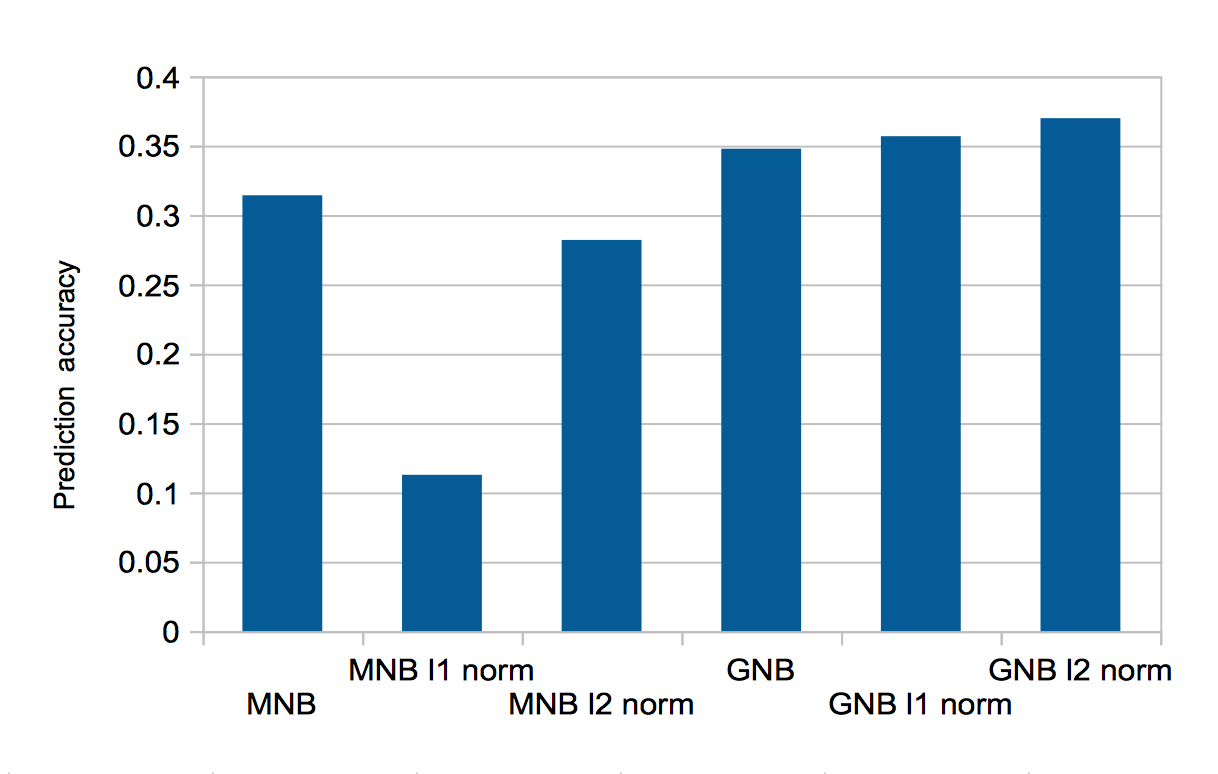
\includegraphics[width=1\columnwidth]{graphs/gnb_param.png}  
\caption{Accuracy versus different Naive Bayes using the original data, $L1$-normalized data, and $L2$-normalized data (train set size = 40,000 and test set size = 10,000)}
\label{fig:gnbparam}
\end{figure}


\subsubsection{Multilayer Perceptron}
Initial learning rate is the most important hyper-parameter in terms of optimization. We set the learning rate to decrease with multiplicative factor $80/(epoch+80)$ where $epoch$ is the number training iterations already done. 

Number of hidden units is an important hyper-parameter in terms of model and training criterion. Unsurprisingly, we find that a better result can usually be obtained if the first hidden layer is larger than the input layer.

\subsubsection{Linear Support Vector Machine }
We vary the marge penalty parameter $C$, but given the nature of the data, the parameter does not seem to effect the error rate. We consistently obtain between 33$\%$ and 34$\%$ accuracy with linear SVMs.

\subsubsection{Convolutional Neural Network}
Considering the massive amount of time that is required to train CNNs, 5-fold validation error was not always considered when choosing hyper-parameters. Instead, we relied on a 4:1 split of the dataset. 

We first tried using two convolutional layers, but quickly realized that using three convolutional layers followed by a two fully connected layers, hidden and output layers, seemed to work best. Similarly we used small filter sizes it gave the best early results. 

As such, we did not do proper hyper-parameter search, and used our knowledge of the model and of the data along with optimal results for the original MNIST dataset to guide us. We can see in Figure \ref{fig:conv_train} that most models will converge to some low error. Note that we did not manage to train any model where the training error converged to some lower error than the validation error (both are very close, as such they are not shown in the figure), and conclude that we could train much larger models before overfitting occurs. Unfortunately, the required training time for such models prohibits us from trying here.
\begin{figure} 
\centering
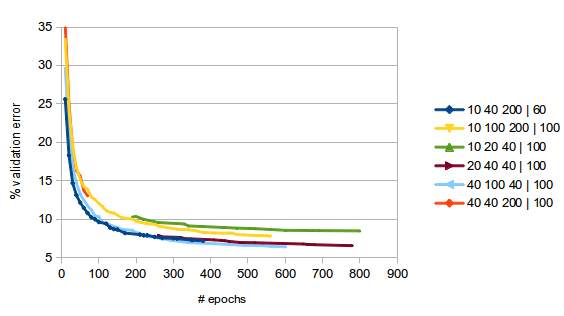
\includegraphics[width=1\columnwidth]{graphs/conv_train.png}  
\caption{Validation error rate of different CNN model sizes during training}
\label{fig:conv_train}
\end{figure}

\subsection{Testing Results Analysis}
We provide further analysis on testing and validation results with help of figures and confusion matrices. We still divide the analysis into four parts based on four algorithms.

\subsubsection{Baseline: Naive Bayes}
We also present the confusion matrix corresponding to the Gaussian Naive Bayes algorithm running with 5-fold cross validation on $L2$ normalized data in Figure \ref{fig:gnb_cm}. We normalized the row vectors of the confusion matrix so that we could make fair comparison among different classes. As can be seen from the normalized confusion matrix, the GNB classifier is capable of distinguish $0$ and $1$ from the others, but it performs relatively poor when classifying $2$ to $7$. Its comparatively promising performance on classifying $0$ may be due to the fact that the digit $0$ is least susceptible to all artificial alterations imposed on the original MNIST dataset (especially rotation).
\begin{figure} 
\centering
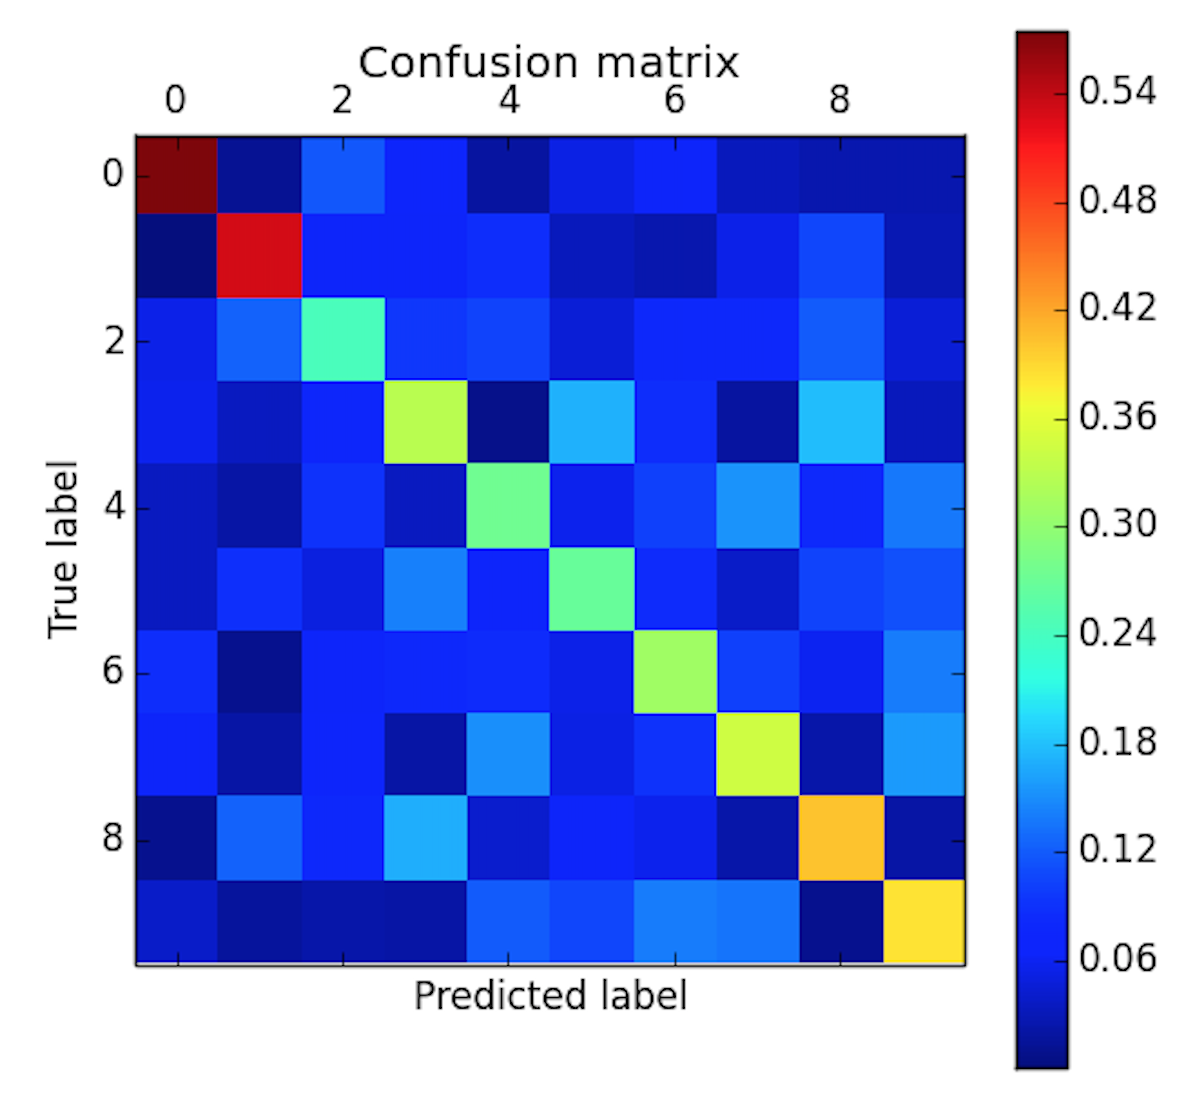
\includegraphics[width=0.8\columnwidth]{graphs/gnb_cm1.png}  
\caption{Normalized confusion matrix for Gaussian Naive Bayes with train set size = 40,000 and test set size = 10,000}
\label{fig:gnb_cm}
\end{figure}


\subsubsection{Multilayer Perceptron}
results of NN

\subsubsection{Linear Support Vector Machine }
The row normalized confusion matrix for Linear Support Vector Machine is given in Figure \ref{fig:lsvm_conf}. Similarly to GNB, LSVM seems to classify well $0$ and $1$, but rather poorly the other classes, probably for the same reasons. 
\begin{figure} 
\centering
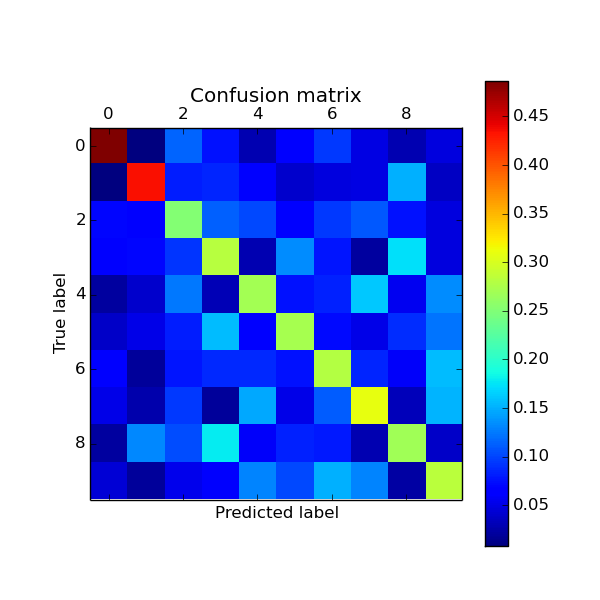
\includegraphics[width=0.9\columnwidth]{graphs/svm_conf.png}  
\caption{ Normalized confusion matrix for LSVM with train set size = 40,000 and test set size = 10,000}
\label{fig:lsvm_conf}
\end{figure}

\subsubsection{Convolutional Neural Network}
We see in Figure \ref{fig:conv_conf} that the ConvNet has good accuracy accross classes. As mentionned earlier, better accuracy could probably be reached with larger model, as the ones we trained would not have a much lower training error than validation error (at most 2$\%$ lower, often less).
\begin{figure} 
\centering
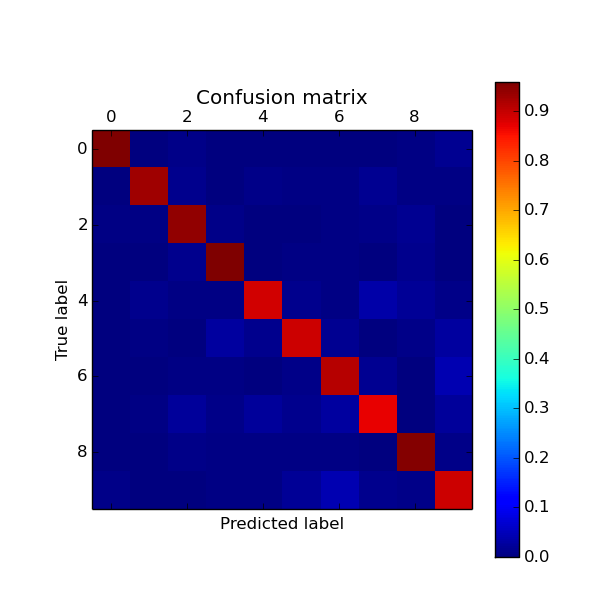
\includegraphics[width=0.9\columnwidth]{graphs/conv_conf.png}  
\caption{Normalized confusion matrix for Convolutional Neural Nets with train set size = 40,000 and test set size = 10,000}
\label{fig:conv_conf}
\end{figure}


\section{Discussion}
The artificial alteration imposed on the MNIST handwritten digit dataset brings about a great amount of noise and complicates the classification task. Many typical machine learning algorithms are not suitable for this modified dataset anymore. For example, Naive Bayes can only achieve up to  $40 \%$ accuracy, even with Gaussian Naive Bayes and many refined preprocessing methods.  More elaborate feature selection and preprocessing techniques may be capable of improving the prediction accuracy using Naive Bayes, but it appears to us that it is unfeasible to achieve an accuracy as high (above $80 \%$) as other more sophisticated algorithms in deep learning.

On the other hand, deep learning models, in particular convolution neural networks, acheive much higher accuracy. Convolutional models take full advantage of the graphical nature of the input space and the high correlation between local visual features, and as such are capable of great scores on this particular task, with little need for feature preprocessing.

To summarize, we endeavoured to classify the modified handwritten digits using four different algorithms. While some are capable of  achieving surprisingly high accuracy,  some illustrate the limitation of "shallow" algorithms. After all, machine learning problems can never be unraveled using a same fixed method. Instead, it requires the exploration of versatile tools, and that is where the charm of machine learning lies.


We	hereby	state	that	all	the	work	 presented	in	this	report	is	that	of	the	authors
\bibliographystyle{abbrv}
\bibliography{sigproc}  

\end{document}
